\documentclass[11pt,twoside,lineno]{GSA_format}
%\documentclass[10pt,twoside,lineno, twocolumn]{GSA_format}
% Use the documentclass option 'lineno' to view line numbers
\usepackage[normalem]{ulem}
\usepackage{float}
\usepackage{amsmath,amssymb}
%\usepackage[textwidth=25cm]{geometry}
\usepackage{siunitx}
\usepackage{arydshln}
\usepackage{graphicx}

\useunder{\uline}{\ul}{}
\articletype{inv} % article type

\newcommand{\bm}[1]{\mbox{\boldmath{$#1$}}}

\newcommand{\beginsupplement}{%
        \setcounter{table}{0}
        \renewcommand{\thetable}{S\arabic{table}}%
        \setcounter{figure}{0}
        \renewcommand{\thefigure}{S\arabic{figure}}%
     }
\title{Patterns of nucleotide diversity under background selection and evolving recombination rates}

\author[$\ast$]{Tom R. Booker}
%\author[$\ast$]{Kartje}
%\author[$\ast$]{Tigano}
%\author[$\ast$]{Whitlock}
%\author[$\ast$]{Payseur}

\affil[$\ast$]{University of British Columbia}

\keywords{Evolutionary Genetics, Population Genetics}

\runningtitle{Background selection and recombination rate evolution} % For use in the footer 

\runningauthor{Booker et al...}

\begin{abstract}
\textit{I'm just using the GENETICS template because it looks nice!}

%The removal of deleterious variants by purifying selection can influence evolution at linked neutral sites in a process called background selection. Recombination decouples neutral and selected sites, so genomic regions that experience high recombination rates minimising the effects of background selection. 


%Background selection, the influence of purifying selection on linked neutral, is likely ubiquitous in evolution. Analysis of genetic data under models of selection at linked sites typically assume that recombination rates are constant over the timescale relevant for patterns of genetic diversity to be influenced. However, recombination is a highly variable trait within and between species so perhaps recombination rate evolution occurs at time scales relevant to models of background selection. In this study, we show using simulations that the change in nucleotide diversity after recombination rates evolve is \\



\end{abstract}

\begin{document}
\maketitle
%\thispagestyle{firststyle}
\marginmark
\firstpagefootnote


%\correspondingauthoraffiliation{1}{Corresponding author: booker@zoology.ubc.ca}
\vspace{-33pt}% Only used for adjusting extra space in the left column of the first page

\section{Introduction}

Natural selection influences the frequencies of genetic variants that affect their carriers' fitness as well as neutral alleles linked to selected sites. The extent by which natural selection at one site influences linked sites depends on the rate of mutations that affect fitness and the rate of recombination. Of the mutations that influence fitness, the majority are likely deleterious with a comparatively small proportion being beneficial (REFS). When deleterious mutations occur they may removed through purifying selection and this can cause linked neutral variants may be lost along with them through a process referred to as background selection (BGS)(Charlesworth et al 1993). Alternatively, as beneficial alleles spread to high frequency, linked neutral variants may hitchhike along with them in a process known as a selective sweep. The effects of both BGS and selective sweeps on a particular neutral locus depend on the rate of recombination between the neutral site and the sites subject to selection (REFS). Indeed, theoretical models of background selection and selective sweeps have provided evolutionary biologists with a framework for understanding natural selection through the analysis of genome-wide patterns of nucleotide diversity. \\

The first empirical evidence that selection at linked sites influences genetic variation across the genome came from studies in \textit{Drosophila}. Aguadé et al (1989) measured genetic variability in the \textit{yellow-achaete-scute} regions located at the tip of the X-chromosome. The \textit{yellow-achaete-scute} regions experience restricted crossing-over and Aguadé et al (1989) found that they harbour far less genetic variation than had been reported for more highly recombining regions of the genome. Aguadé et al (1989) suggested that selective sweeps (though that term was not coined until later), which reduce nucleotide diversity ($\pi$) to the greatest extent in regions of restricted recombination, potentially explained their findings. Begun and Aquadro (1992) then showed that there is a clear correlation between recombination rate and nucleotide diversity ($\pi$) using loci sampled from across the \textit{D. melanogaster} genome. Furthermore, Begun and Aquadro (1992) showed that there was little evidence for a correlation of between-species divergence and recombination rate, which one might expect if recombination were itself mutagenic. By fitting a model of selective sweeps to the observed correlation between $\pi$ and recombination rate, Wiehe and Stephan (1993) made inferences about the rate and strength of beneficial mutations. Around the same time, however, Charlesworth et al (1993) demonstrated that BGS could also potentially explain the correlation between $\pi$ and the recombination rate. In the time since these papers were published, many studies have used the relationship between nucleotide diversity and recombination rate to make inferences about the strength of selection and the rate at which selected mutations occur (REF DUMP). \\

Interpreting patterns of genetic variability in terms of selection at linked sites relies on accurate estimates of recombination rates. Additionally, there is an implicit assumption that the landscape of recombination evolves slowly and can be considered invariant over the timescale relevant for patterns of diversity to be influenced by selection. Empirical estimates of recombination rates can be obtained by examining the inheritance of genetic markers through known pedigrees, as in traditional genetic mapping, or by directly comparing an individual's genome to the the genomes of its gametes (REF). Both methods provide estimates of recombination in contemporary population, but if recombination rates evolve rapidly, empirical recombination rate estimates may not reflect patterns of nucleotide diversity that were influenced by the ancestral recombination rate landscape.\\

There is reason to think that recombination rate landscapes have evolved rapidly in some lineages. In the house mouse (\textit{Mus musculus}), for example, there has likely been extensive evolution of recombination rate landscape in the last five million years. It is estimated that \textit{Mus musculus} (2\textit{n}=40) and \textit{Mus pahari} (2\textit{n}=48) began to diverge around 5 million years ago and in that time approximately 18 large syntenic breaks accumulated in the lineage leading to \textit{M. musculus} (Thybert et al 2018). Due to the requirement of at least one cross-over per meiosis in mammals, an increase or a decrease in the length of a chromosome will necessarily influence the recombination rate. Thus karyotype evolution has likely influenced recombination rate landscapes at broad scales in \textit{Mus musculus}. More recently, the \textit{M. musculus} lineage began to diverge into the M. musculus species complex (REFS), and differences in the genome-wide rate of recombination have arisen amongst the members of this group (Dumont and Payseur XXXX). Finally, Recombination in mice is typically restricted to narrow windows  of the genome (on the order of 10,000 basepairs) referred to as recombination hotspots (REFS). The location of recombination hotspots in mice, as in humans and several other mammals (REF), are determined by the binding of a zinc-finger protein encoded by the PRDM9 gene to specific DNA motifs (REFS). There is evidence that PRDM9 has undergone numerous bouts of positive selection (Kono et al 201X) and natural populations of \textit{M. musculus spp.} harbour numerous PRDM9 alleles corresponding to varying suites of recombination hotspots  (Smagulova et al 2015). Overall, there is clear evidence that recombination rates have evolved at broad and fine scales in mice. \\

In lineages that have experienced recent evolution of the recombination rate landscape the hallmark signature of selection at linked sites, a positive correlation between nucleotide diversity and recombination rate may be obscured. In this paper, we examine how patterns of neutral genetic variability under background selection respond to evolution of the recombination rate. We make use of a previously derived function that describes coalescence times after instantaneous population size change to model the effects of background selection on neutral genetic diversity after a change in the recombination rate. We demonstrate how evolution of the recombination rate at both broad and fine scales may influence the correlation between nucleotide diversity and recombination rate using simulations. Finally, we re-analyse results from Kartje et al (2020) on the correlation natural \textit{Mus musculus domesticus} and find a pattern that suggests recombination rate evolution has obscured the patterns of selection at linked sites in that species.




\section{Results}

Evolution of the recombination rate causes a change in the effects of background selection that resembles a change in the effective population size (Figure \ref{fig:BGS_over_time_fixed_s}). 



\begin{figure}[H]
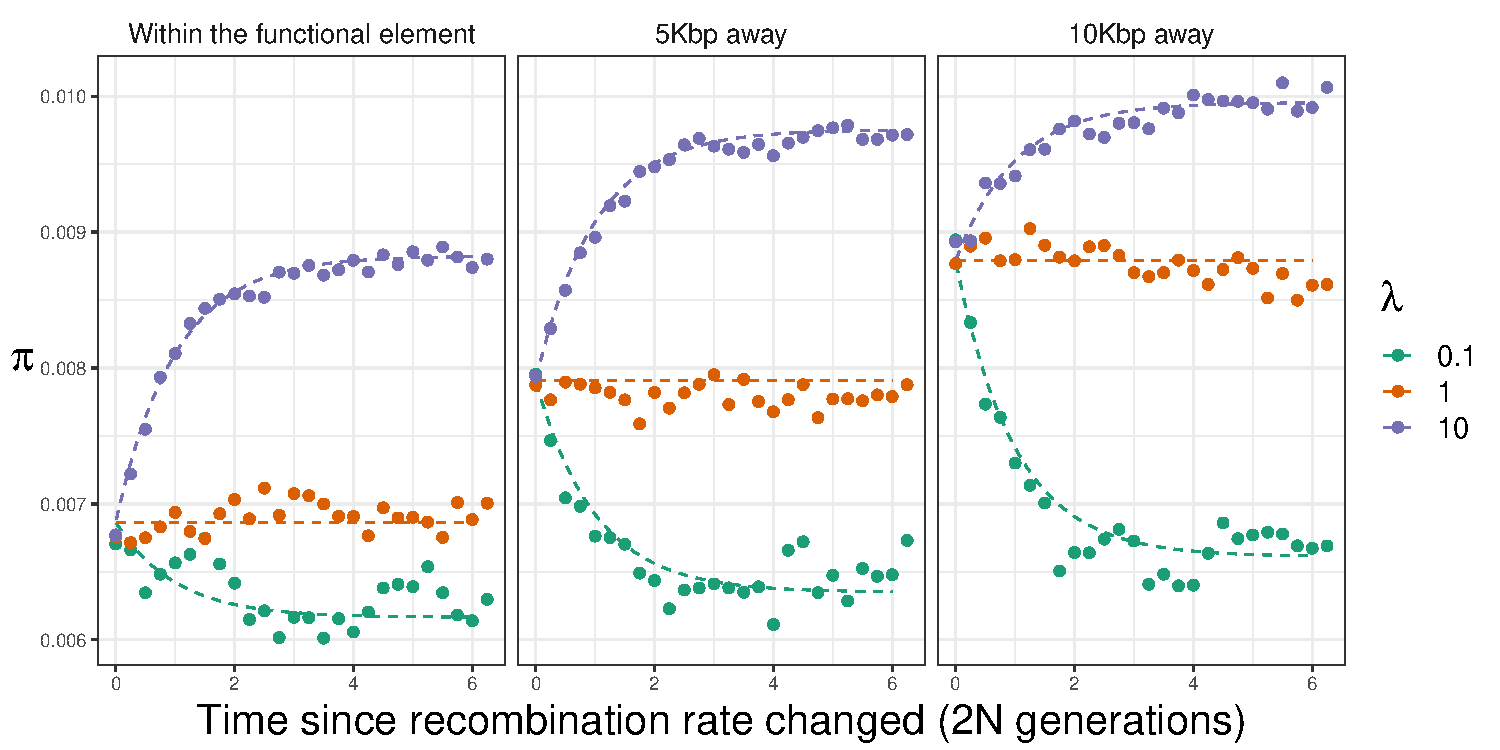
\includegraphics[width=\textwidth]{../TheoreticalExpectation/B_over_time_fixed_s_plot}
\caption{Nucleotide diversity over time after recombination rates change by a factor $\lambda$ for neutral sites in or around a functional element. The dashed lines were calculated using Equation \ref{BGS_rec}.}
\label{fig:BGS_over_time_fixed_s}
\end{figure}

An instantaneous change in the recombination landscape may 

\begin{figure}[H]
\includegraphics[ height=0.4\textheight]{../Plots/simpleMap03_pi_r_correlationOverTime.pdf}
\caption{Spearman's correlation between nucleotide diversity ($\pi$) and recombination rate ($r$) over time after recombination rates evolve. Panel A shows results for 10 Kbp, 100 Kbp and 1Mbp analysis windows. } 
\end{figure}


\begin{figure}[H]
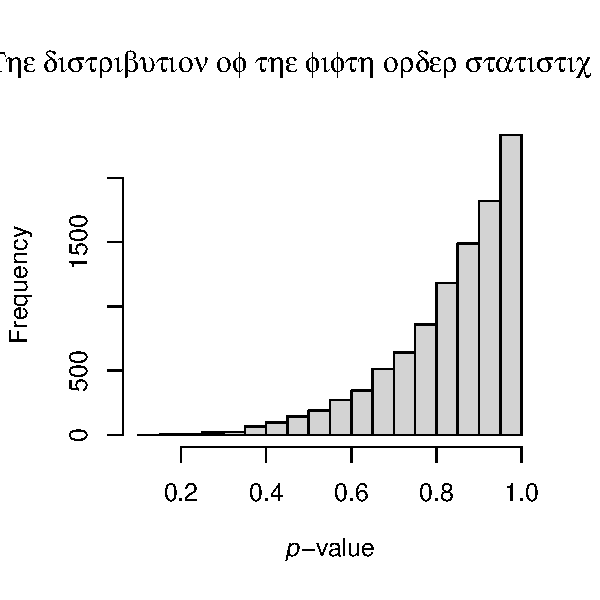
\includegraphics[ height=0.4\textheight]{../Plots/pi_r_correlationOverTime.pdf}
\caption{Spearman's correlation between nucleotide diversity ($\pi$) and recombination rate ($r$) over time after recombination rates evolve. Panel A shows results for 10 Kbp, 100 Kbp and 1Mbp analysis windows. } 

\end{figure}


\section{Discussion}

Here is an erudite description of the results and what we can infer from them. \\

For the sake of simplicity, in the model we used and the simulations we performed, we assumed that recombination rates evolve instantaneously. While that is obviously an oversimplication, there is reason to expect that recombination rate changes may evolve rapidly. Chromosomal fusions may exhibit meiotic drive (REFS) and so may rapidly rise to fixation in a population 

Cutter and Payseur (2012) noted that numerous species that have been examined do not exhibit a positive correlation between diversity and recombination rate. For example, wild and domesticated rice species (\textit{Oryza rufipogon} and \textit{Oryza sativa}, respectively) exhibit negative correlations between diversity and recombination rate (Flowers et al 2011).



\begin{table*}[t]
\
\resizebox{\textwidth}{!}{\begin{tabular}{cc|
           *{2}{S[round-mode = figures,
            round-precision = 3]}|
                 *{2}{S[round-mode = figures,
            round-precision = 3]}|
                 *{2}{S[round-mode = figures,
            round-precision = 3]}}
                 \hline
 & & \multicolumn{2}{c}{Whole Genome} & \multicolumn{2}{c}{Conserved Chromosomes}& \multicolumn{2}{c}{Non-Conserved Chromosomes}\\
 {Window} & {Population} &  {Spearman`s $\rho$} & {$p$-value} &{Spearman`s $\rho$} & {$p$-value} & {Spearman`s $\rho$} & {$p$-value}\\ 
  \hline
5Kbp& Gough Island & 0.00766946556467726 & \num{4.28487483542177e-05} & 0.00879560871962056 & 0.0102132179985377 & 0.00485568404015206 & 0.0301693742321603 \\ 
  5Kbp & France & 0.00408044307052427 & 0.0294929095581957 & 0.0402631172537313 & \num{6.10313340830373e-32} & -0.0107049632666829 & \num{1.75806407865671e-06} \\ 
  5Kbp & Germany &  0.00752167382031877 & \num{6.05264156648312e-05} & 0.0151531276721775 & \num{9.6335227129151e-06} & 0.00386135398506519 & 0.0849380013628119 \\ 
  1Mbp & Gough Island &  0.0535515289545324 & 0.00946379855975982 & 0.0588327090738239 & 0.124246200526924 & 0.043697649001863 & 0.0748313470537267 \\ 
  1Mbp & France &  0.0449712235482249 & 0.0293606123894296 & 0.134981255195878 & 0.000400166310010629 & 0.00998569897732337 & 0.684066944892074 \\ 
  1Mbp & Germany &  0.0535221710805316 & 0.00953371381645413 &  0.0774668203290588 & 0.0428305229197646 & 0.0425693100291219 & 0.0828457161038532 \\ 
\hline
\end{tabular}}

\caption{The correlation between nucleotide diversity ($\pi$) and recombination rate for three populations of house mice (\textit{Mus musculus domesticus}) calculated from all autosomes, conserved chromosomes that exhibit no syntenic breaks between \textit{M. musculus} and \textit{M. pahari} and the non-conserved chromosomes as identified by Thybert et al (2018).}
\label{Table1}
\end{table*}



Cicconardi et al (2020) demonstrated a clear relationship between chromosome size and putatively neutral diversity in \textit{Heliconius} butterflies. Between 


We re-analysed the correlation between $\pi$ and $r$ in \textit{Mus musculus domesticus} using previously analysed data from Kartje et al (2020) (Table \ref{Table1}). 

%We modelled evolution of the recombination rate as an instantaneous change. While an instantaneous change is obviously unrealistic, recombination rate modifiers may rapidly go fixation. There is evidence that karyotypic variants such as Robertsonian fusions that act as meiotic drivers (REF), and such drivers can reach 


\section{Methods}
\subsection{Model}
Background selection has been modelled as the reduction in effective population size ($N_e$) at a neutral site due to the removal of deleterious variants. The effects of background selection are often expressed as $B = \frac{N_e}{N_0}$, where $N_e$ is the effective population size and $N_0$ is the expected population size under strict neutrality. In a non-recombining genome, $B$ is proportional to the ratio of the deleterious mutation rate to the strength of selection acting on harmful mutations (Charlesworth et al 1993). For a neutral site present on a recombining chromosome, the effects of background selection depend on the density of functional sites (i.e. those that can mutate to generate deleterious alleles), the mutation rate, the strength of selection and the recombination rate (Hudson and Kaplan 1995; Nordborg et al 1996; Nordborg 1997). For a neutral locus $\nu$ linked to $x$ functional sites, the reduction in $N_e$ has been described with the following equation:

\begin{equation}
B_{\nu} = \frac{N_e}{N_0} = exp[ -\sum\limits_x \frac{u_x}{t(1+(1-t)r_{x,v}/t)^2} ]
\label{nordborg}
\end{equation}\noindent
Where $u_x$ is the deleterious mutation rate at functional site $x$, $t$ is the heterozygous fitness effect of a deleterious mutation (i.e. 0.5$s$ in the case of semi-dominance) and $r_{x,\nu}$ is the recombination map distance between the neutral locus and functional site $x$. In the above equation, deleterious mutations have fixed effects, but it is straightforward to incorporate a distribution of fitness effects (Nordborg et al 1996). The above equation holds when selection is sufficiently strong  such that random drift does not overwhelm selection ($N_es > 1$) (Good et al 2014). \\

When the recombination rate landscape evolves it may cause a change in the effects of BGS in particular genomic regions. We modelled the time it takes for coalescence times, or patterns of nucleotide diversity, to reflect background selection expected under a new recombination rate regime using expressions formulated to describe coalescence times after a population size change. For a neutral site $\nu$, the combined effects of recombination, mutation and purifying selection cause there to be a reduction of $B_{\nu,1}$ to coalescence times. At time $T_0$ in the past (in $2N_e$ generations), the population underwent an instantaneous change in the recombination rate so $\nu$ now experiences a BGS effect of $B_{\nu,2}$. We modified an expression for coalescence times after an instantaneous population size change from Johri et al (2020), to obtain the following equation,

\begin{equation}
B_{\nu,\Delta r} = B_{\nu,2} ( 1 + (\frac{B_{\nu,1}}{B_{\nu,2}} - 1)e^{-T_0})
\label{BGS_rec}
\end{equation}
\noindent
Note that Equation X from Pool and Nielsen (2009) provided similar expressions to those given in Johri et al (2020). 


\subsection{Simulations}

We simulated BGS under recombination rate evolution using two types of simulations in \textit{SLiM} v3.2 (Haller et al 2018). In all cases, diploid populations of $N$ = 1,000 individuals were simulated. \\

The first set of simulations was designed to examine how long it takes for patterns of neutral diversity under BGS to equilibrate after the recombination rate evolves. In these simulations, the genome was 25Kbp long with a 5Kbp functional element in the centre. Mutations occurred in the functional element at rate $\mu = 2.5\times10^{-6}$ and had semi-dominant fitness effects with a fixed selection coefficient of -0.05. We also simulated cases with varying fitness effects using a gamma distribution with mean ($\bar{s}$) of -0.1 and a shape parameter of 0.1. Recombination occurred at a uniform rate of $r = 2.5\times10^{-6}$ across the chromosome. After 15,000 generations, we simulated an instantaneous change in the recombination rate, multiplying $r$ by $\lambda$, giving $r = \lambda2.5\times10^{-6}$. We simulated cases with $\lambda$ = 0.1, 1.0 and 10.0. Simulated populations were sampled every 500 generations after the recombination rate changed and we performed 200 replicates for each set of parameters tested. Note that these simulations were not designed to be particularly realistic, but to provide clear cut patterns to test the theoretical predictions. \\

The second set of simulations was designed to examine how patterns of $\pi$ versus $r$ varied over time when recombination rates evolved at fine and/or broad scales. For these simulations, we modelled chromosomes that were 10Mbp long. Deleterious mutations occurred at random across the length of the sequence at a rate of $1\times10^{-7}$ with semi-dominant fitness effects drawn from a gamma distribution with a mean ($\bar{s}$) of -0.1 and a shape parameter of 0.1. Populations evolved under background selection for 15,000 generations  \\

We modelled the evolution of hotspots in the following way. At the beginning of a simulation, a Poisson number of hotspots was sampled with an expectation of 60, which was based on the average number of double-strand break hotspots observed by Smagulova et al (2015). Locations for 10,000bp hotspots were then sampled across the simulated chromosome. Recombination occurred at a uniform rate of $r=2.08\times10^{-7}$ except in hotspots where it occurred at a rate of $r=2.08\times10^{-5}$. These rates were chosen to give an overall recombination rate similar to that of a chromosome that recombined at a uniform rate of $r=2.5\times10^{-6}$. \\

We modelled recombination rate evolution at broad scales in the following way. The genome-wide average recombination rate in \textit{Mus musculus} is XXX cM\/Mbp. The distribution of recombination rates is approximately normal with mean XXX cM\/Mbp and variance YYY. We scaled recombination in these simulations to simulate a large natural population using a comparatively small number of individuals in \textit{SLiM}. At the beginning of a simulation, we sampled  10 recombination rates from a normal distribution (mean scaled\_XXX, variance scaled\_YYY). As above, we generated a new recombination map after 15,000 generations of evolution, sampled the population then continued to sample the population every 
we generated a new set of recombination hotspots as above and sampled the population every 500 generations for a further 3,000 generations. \\

For all simulations, we used the tree sequence recording option in \textit{SLiM} and neutral mutations were added to the resulting tree-sequences at a rate of 2.5$\times10^{-6}$ using PySLiM (version XX). Nucleotide diversity ($\pi$) was calculated in windows of varying size using sci-kit-allel (version X.Y, Citation).

\beginsupplement
\section{Supplementary Material}

\begin{figure}[h]
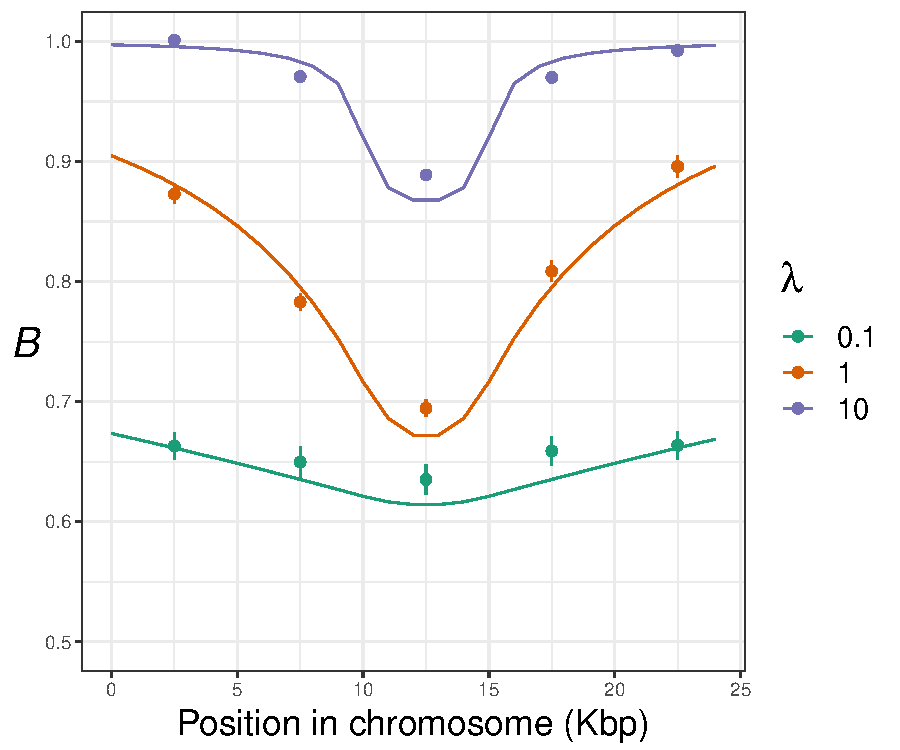
\includegraphics[width=\textwidth]{../TheoreticalExpectation/B_fixed_plot}
\caption{The effects of background selection across simulated chromosomes. \textit{B} was calculated for simulated data by comparing observed $\pi$ to the neutral expectation of $4N_e\mu=0.01$. The lines show the theoretical expectation calculated using formulae from Nordborg et al (1996).}
\label{fig:BGS_fixed_plot}
\end{figure}

\end{document}


The first empirical evidence that selection at linked sites influences genetic variation across the genome came from studies in \textit{Drosophila}. Aguadé et al (1989) measured genetic variability in the \textit{yellow-achaete-scute} regions located at the tip of the X-chromosome. The \textit{yellow-achaete-scute} regions experience restricted crossing-over and Aguadé et al (1989) found that they harbour far less genetic variation than had been reported for more highly recombining regions of the genome. Aguadé et al (1989) suggested that selective sweeps (though that term was not coined until later), which reduce nucleotide diversity ($\pi$) to the greatest extent in regions of restricted recombination, potentially explained their findings. Begun and Aquadro (1992) then showed that there is a clear correlation between recombination rate and nucleotide diversity ($\pi$) using loci sampled from across the \textit{D. melanogaster} genome. Furthermore, Begun and Aquadro (1992) showed that there was little evidence for a correlation of between-species divergence and recombination rate, which one might expect if recombination were itself mutagenic. Soon afterwards, Charlesworth et al (1993) demonstrated that background selection could also potentially explain the correlation between $\pi$ and the recombination rate.  \\